% =============================================================================
% Chapter 2: Biological Basis : Pit Viper Thermal Sensing System
% Pit-Viper-Inspired Infrared-Thermal and Visual Sensor Fusion
% for Nocturnal UAV Navigation
% =============================================================================
\selectlanguage{hebrew}

\section{בסיס ביולוגי: מערכת החוש התרמי של הצפע הגומתי}
\label{sec:ch02_bio_basis}

\subsection{אנטומיה ופיזיולוגיה של איבר הגומה}
\label{sec:ch02_pit_organ}

הצפע הגומתי (\emph{Crotalus cerastes}) הוא נחש מדברי השייך למשפחת הצפעיים (\emph{Viperidae}) ותת-משפחת הצפעוניים (\emph{Crotalinae}), הכוללת את הנחשים בעלי איבר הגומה. איבר הגומה (\en{pit organ}) הוא חיישן תרמי ייחודי הממוקם בין העין לנחיר בכל צד של הראש. איבר זה התפתח כהתאמה אבולוציונית לציד לילי, ומאפשר לנחש לזהות טרף בעל דם חם גם בחושך מוחלט \cite{Simmons1979BatSonar}.

מבנה איבר הגומה מורכב משקע גרמי בעומק של כ-5 מ\"מ, שבתחתיתו קרום דקיק בעובי של כ-15 $\mu$m. קרום זה מכיל כ-7,000 תאי קולטן תרמיים הרגישים לשינויי טמפרטורה קטנים עד 0.003$^{\circ}$C. הקרום מתוח על פני השקע כמו עור תוף, ומגיב לקרינת אינפרה-אדום הנקלטת דרך פתח קטן בקוטר של כ-1 מ\"מ. הפתח מכוון קדימה ומטה, ומספק שדה ראייה של כ-60 מעלות אופקית ו-30 מעלות אנכית \cite{Schnitzler1968DSC}.

מנגנון הקליטה התרמית מבוסס על עקרון הקרינה התרמית. כל עצם בטמפרטורה מעל האפס המוחלט פולט קרינה אלקטרומגנטית בתחום האינפרה-אדום, שעוצמתה פרופורציונלית ל-$T^4$ על פי חוק סטפן-בולצמן. איבר הגומה רגיש במיוחד לקרינה בתחום 8-12 $\mu$m, התואם לשיא הקרינה של גוף בטמפרטורה של 300 K (טמפרטורת גוף של יונקים). רגישות ספקטרלית זו מאפשרת לנחש לזהות הבדלי טמפרטורה קטנים בין טרף חם לסביבה קרה.

\subsection{עיבוד עצבי של מידע תרמי}
\label{sec:ch02_neural_processing}

המידע התרמי מאיבר הגומה מעובד במוח הנחש במסלול עצבי ייעודי. תאי הקולטן בקרום הגומה שולחים אקסונים לגנגליון העצבי הממוקם בסמוך לאיבר. מהגנגליון, הסיבים העצביים מובילים לגרעין התרמי במוח התיכון (\en{mesencephalic nucleus}), שם מתבצע עיבוד ראשוני של המידע התרמי. משם, המידע מועבר לקורטקס האופטי (\en{optic tectum}) ולקורטקס הסומטוסנסורי (\en{somatosensory cortex}), שם הוא משולב עם מידע חזותי מהעיניים \cite{Schuller1974DSC}.

מחקרים אלקטרופיזיולוגיים הראו כי תאי עצב בקורטקס האופטי של הצפע מגיבים לגירויים תרמיים וחזותיים כאחד. תאים אלה, המכונים תאים דו-מודאליים (\en{bimodal neurons}), מאפשרים אינטגרציה של מידע משני החושים ברמה העצבית. מנגנון אינטגרציה זה הוא הבסיס העצבי ליכולתו של הנחש לנווט ולצוד בתנאי חושך מוחלט.

העיבוד העצבי של המידע התרמי כולל מספר שלבים: (1) זיהוי שינויי טמפרטורה מהירים, המאפשר זיהוי תנועת טרף; (2) נורמליזציה לטמפרטורת הסביבה, המאפשרת זיהוי עצמים חמים גם בסביבה חמה; (3) מיפוי מרחבי של שדה הטמפרטורה, המאפשר זיהוי מיקום מדויק של מקור החום; (4) אינטגרציה עם מידע חזותי, המאפשרת זיהוי עצמים גם כאשר אחד החושים אינו מספק מידע מספק.

\subsection{מיפוי חום כמפת סליאנס ביולוגית}
\label{sec:ch02_saliency}

אחד המנגנונים המרכזיים במערכת הראייה של הצפע הוא זיהוי עצמים בעלי טמפרטורה שונה מהסביבה. מנגנון זה, המכונה מיפוי חום תרמי (\en{thermal saliency mapping}), מאפשר לנחש לזהות טרף חם על רקע קר, או מכשולים קרים על רקע חם. המיפוי מבוסס על ניגודיות תרמית, המוגדרת כהפרש הטמפרטורה בין העצם לסביבתו.

מחקרים התנהגותיים הראו כי הצפע מסוגל לזהות ניגודיות תרמית של 0.1$^{\circ}$C בלבד במרחק של עד 1 מטר. רגישות זו מאפשרת לו לזהות טרף קטן כעכבר במרחק של מספר מטרים, גם כאשר הטרף מוסתר מתחת לעלים או בחול. יכולת זו היא קריטית להישרדותו של הנחש בסביבה המדברית הקשה.

המיפוי התרמי במוח הנחש יוצר ייצוג מרחבי של שדה הטמפרטורה בסביבה, בדומה למפת חום (\en{heat map}). אזורים בעלי ניגודיות תרמית גבוהה מסומנים כבעלי סליאנס גבוה, ומעוררים תגובה עצבית חזקה יותר. מנגנון זה מאפשר לנחש להתמקד בעצמים רלוונטיים תוך סינון רעש תרמי מהסביבה.

\subsection{אינטגרציה רב-חושית במוח הנחש}
\label{sec:ch02_multi_sensory}

האינטגרציה הרב-חושית במוח הנחש היא אחד המנגנונים המרתקים ביותר במערכת הראייה שלו. מידע חזותי מהעיניים ומידע תרמי מאיבר הגומה מעובדים במקביל ומשולבים לייצוג מאוחד של הסביבה. מחקרים הראו כי האינטגרציה מתרחשת בשני שלבים: ברמה התאית, באמצעות תאים דו-מודאליים המגיבים לשני סוגי הגירויים; וברמת הרשת, באמצעות קשרים עצביים בין האזורים החזותיים והתרמיים במוח.

מנגנון האינטגרציה מאפשר לנחש להתמודד עם מצבים בהם אחד החושים אינו מספק מידע מספק. לדוגמה, בתנאי חושך מוחלט, המידע החזותי מוגבל, אך המידע התרמי מספק תמונה מלאה של הסביבה. לעומת זאת, בתנאי תאורה טובים, המידע החזותי מספק רזולוציה מרחבית גבוהה יותר, והמידע התרמי משמש כחיישן משלים.

האינטגרציה הרב-חושית במוח הנחש מהווה מודל חישובי למערכות מיזוג חיישנים מלאכותיות. העקרונות הביולוגיים של אינטגרציה זו, הכוללים מיפוי חום תרמי, נורמליזציה לטמפרטורת הסביבה, ואינטגרציה עם מידע חזותי, מהווים בסיס תאורטי לאלגוריתמי המיזוג שפותחו במחקר זה.

\subsection{השלכות למערכות ניווט אוטונומיות}
\label{sec:ch02_implications}

העקרונות הביולוגיים של מערכת הראייה התרמית של הצפע הגומתי מספקים תובנות חשובות לתכנון מערכות ניווט אוטונומיות ליליות. ראשית, השימוש במפת חום תרמית כמפת סליאנס מאפשר זיהוי מכשולים גם בתנאי חושך מוחלט, בדומה לאופן שבו הנחש מזהה טרף חם על רקע קר. שנית, האינטגרציה הרב-חושית במוח הנחש מדגימה כיצד ניתן לשלב מידע משני חיישנים שונים לייצוג מאוחד של הסביבה.

בפרקים הבאים של מאמר זה, אנו מממשים עקרונות ביולוגיים אלה במסגרת חישובית מלאה. פרק 3 מתאר את מערך החיישנים והכיול המשותף, המאפשר רישום מרחבי וזמני מדויק בין המצלמה החזותית לתרמית. פרק 4 מציג את מסגרת ה-\en{SLAM} ההיברידית, המשלבת מידע משני החיישנים בארכיטקטורת גרף-\en{SLAM}. פרק 5 מתאר את מנגנון המיזוג הרב-שכבתי, המממש אינטגרציה רב-חושית ברמות שונות של עיבוד מידע.

\subsection{מודל מתמטי של רגישות תרמית}
\label{sec:ch02_thermal_sensitivity_model}

כדי להעביר את העקרונות הביולוגיים למערכת חישובית, נפתח מודל מתמטי של רגישות איבר הגומה. הקרינה התרמית הנקלטת באיבר הגומה מעצם בטמפרטורה $T_{\text{obj}}$ על רקע בטמפרטורה $T_{\text{amb}}$ מתוארת על ידי חוק סטפן-בולצמן:

\begin{equation}
P_{\text{det}} = \epsilon \sigma A \l$e$ft( T_{\text{obj}}^4 - T_{\text{amb}}^4 \right)$$ \cdot \tau_{\text{atm}}(d)
\label{eq:ch02_radiation_power}
\end{equation}

כאשר $\epsilon$ היא פליטות העצם, $\sigma = 5.67 \times 10^{-8}$ W/m$^2$K$^4$ הוא קבוע סטפן-בולצמן, $A$ הוא שטח הקרום הקולט, ו-$\tau_{\text{atm}}(d) = \e$x$p(-$$\alpha$$_{\text{atm}} d)$$$ היא העברת האטמוספירה במרחק $d$. עבור שינוי קטן בטמפרטורה $$\Delta$ T = T_{\text{obj}} - T_{\text{amb}}$, ניתן לקרב את ההספק הנקלט על ידי ליניאריזציה סביב $T_{\text{amb}}$:

\begin{equation}
P_{\text{det}} \approx 4 \epsilon \sigma A T_{\text{amb}}^3 \Delta T \cdot \tau_{\text{atm}}(d)
\label{eq:ch02_linearized_power}
\end{equation}

קירוב זה מראה כי ההספק הנקלט פרופורציונלי ל-$\Delta T$, וכי הרגישות $\partial P_{\text{det}} / \partial T \propto T_{\text{amb}}^3$ עולה עם טמפרטורת הסביבה. תוצאה זו מסבירה מדוע הצפע הגומתי, החי בסביבה מדברית חמה, פיתח רגישות תרמית גבוהה במיוחד: טמפרטורת הסביבה הגבוהה מגבירה את הרגישות להפרשי טמפרטורה קטנים.

\subsection{ניתוח השוואתי: מערכת הראייה של הצפע מול מערכות חיישנים מלאכותיות}
\label{sec:ch02_comparative_analysis}

כדי להמחיש את היתרונות של המערכת הביולוגית על פני מערכות מלאכותיות קיימות, נבצע ניתוח השוואתי. טבלה \ref{tab:ch02_comparison} מציגה השוואה בין מאפייני איבר הגומה של הצפע לבין מצלמה תרמית מסחרית טיפוסית (\en{FLIR Boson 640}).

\begin{table}[htbp]
\centering
\caption{השוואה בין איבר הגומה של הצפע הגומתי לבין מצלמה תרמית מסחרית. (Comparison between pit viper pit organ and commercial thermal camera.)}
\label{tab:ch02_comparison}
\adjustbox{max width=\columnwidth}{%
\begin{tabular}{@{}lcc@{}}
\toprule
\textbf{מאפיין} & \textbf{איבר גומה (צפע)} & \textbf{מצלמה תרמית (\en{FLIR Boson 640})} \\
\midrule
רזולוציה מרחבית & $\sim$1000 תאי קולטן & 640x512 פיקסלים \\
רגישות תרמית & 0.003$^{\circ}$C & 0.04$^{\circ}$C (40 mK) \\
שדה ראייה & 60$^{\circ}$ x 30$^{\circ}$ & 50$^{\circ}$ x 40$^{\circ}$ \\
טווח ספקטרלי & 8-12 $\mu$m & 7.5-13.5 $\mu$m \\
זמן תגובה & $\sim$10 ms & $\sim$16.7 ms (60 fps) \\
צריכת הספק & $\sim$0.1 mW (ביולוגי) & 1.8 W \\
משקל & $\sim$0.1 g & 180 g \\
יכולת כיול עצמי & מובנית (אדפטיבית) & דורשת NUC כל 5 דקות \\
\bottomrule
\end{tabular}%
}
\end{table}

הנתונים בטבלה \ref{tab:ch02_comparison} מראים כי איבר הגומה הביולוגי עדיף על המצלמה התרמית המסחרית במספר מאפיינים קריטיים: רגישות תרמית גבוהה פי 13, צריכת הספק נמוכה פי 18,000, ומשקל זניח. לעומת זאת, המצלמה המסחרית מציעה רזולוציה מרחבית גבוהה יותר ושדה ראייה רחב יותר. הפער ברגישות התרמית מדגיש את הפוטנציאל הרב בשיפור טכנולוגיות חיישנים תרמיים מלאכותיים באמצעות השראה ביולוגית.

\subsection{מנגנון נוירו-אדפטיבי: למידה והסתגלות בתנאי סביבה משתנים}
\label{sec:ch02_neuro_adaptive}

אחד המנגנונים המרתקים ביותר במערכת הראייה של הצפע הגומתי הוא היכולת להסתגל לתנאי סביבה משתנים באמצעות מנגנון נוירו-אדפטיבי (\en{neuro-adaptive mechanism}). מחקרים הראו כי רגישות איבר הגומה אינה קבועה, אלא מותאמת באופן דינמי לטמפרטורת הסביבה ולרמת הרעש התרמי. מנגנון זה, המכונה \en{adaptive gain control}, מאפשר לנחש לשמור על רגישות אופטימלית במגוון רחב של תנאי סביבה.

המנגנון הנוירו-אדפטיבי פועל באמצעות משוב עצבי מהקורטקס האופטי לאיבר הגומה. כאשר רמת הרעש התרמי בסביבה גבוהה (לדוגמה, בסביבה מדברית חמה בשעות הצהריים), הרגישות מופחתת כדי למנוע התראות שווא. לעומת זאת, כאשר רמת הרעש נמוכה (לדוגמה, בלילה קר), הרגישות מוגברת כדי לאפשר זיהוי טרף גם במרחק רב. מנגנון זה מתואר מתמטית על ידי פונקציית הרגישות האדפטיבית:

\begin{equation}
$S(T_{\text{amb}}, \sigma_{\text{noise}})$ = S_0 \cdot \frac{\sigma_{\text{noise}}^2}{\sigma_{\text{noise}}^2 + (T_{\text{amb}} - T_0)^2}
\label{eq:ch02_adaptive_sensitivity}
\end{equation}

כאשר $S_0$ היא הרגישות המקסימלית, $\sigma_{\text{noise}}$ היא סטיית התקן של רעש הרקע התרמי, $T_{\text{amb}}$ היא טמפרטורת הסביבה, ו-$T_0$ היא טמפרטורת הייחוס. מודל זה מראה כי הרגישות יורדת ככל שטמפרטורת הסביבה מתרחקת מטמפרטורת הייחוס, ובכך מונעת התראות שווא בסביבות קיצוניות. עיקרון זה מהווה השראה ישירה למנגנון המיזוג האדפטיבי שפותח בפרק 5 של מאמר זה.

\subsection{סיכום}
\label{sec:ch02_summary}

בפרק זה הצגנו את הבסיס הביולוגי של מערכת הראייה התרמית של הצפע הגומתי. תיארנו את האנטומיה והפיזיולוגיה של איבר הגומה, את מנגנון העיבוד העצבי של מידע תרמי, ואת האינטגרציה הרב-חושית במוח הנחש. העקרונות הביולוגיים שהוצגו בפרק זה מהווים בסיס תאורטי לאלגוריתמי המיזוג והניווט שפותחו במחקר זה. פיתחנו מודל מתמטי של רגישות תרמית המסביר את הרגישות הגבוהה של איבר הגומה, וביצענו ניתוח השוואתי המדגים את יתרונות המערכת הביולוגית על פני מערכות מלאכותיות. כמו כן, הצגנו את מנגנון הנוירו-אדפטיבי המאפשר הסתגלות דינמית לתנאי סביבה משתנים, המהווה השראה ישירה למנגנון המיזוג האדפטיבי שפותח במחקר זה.

\begin{figure}[htbp]
\centering
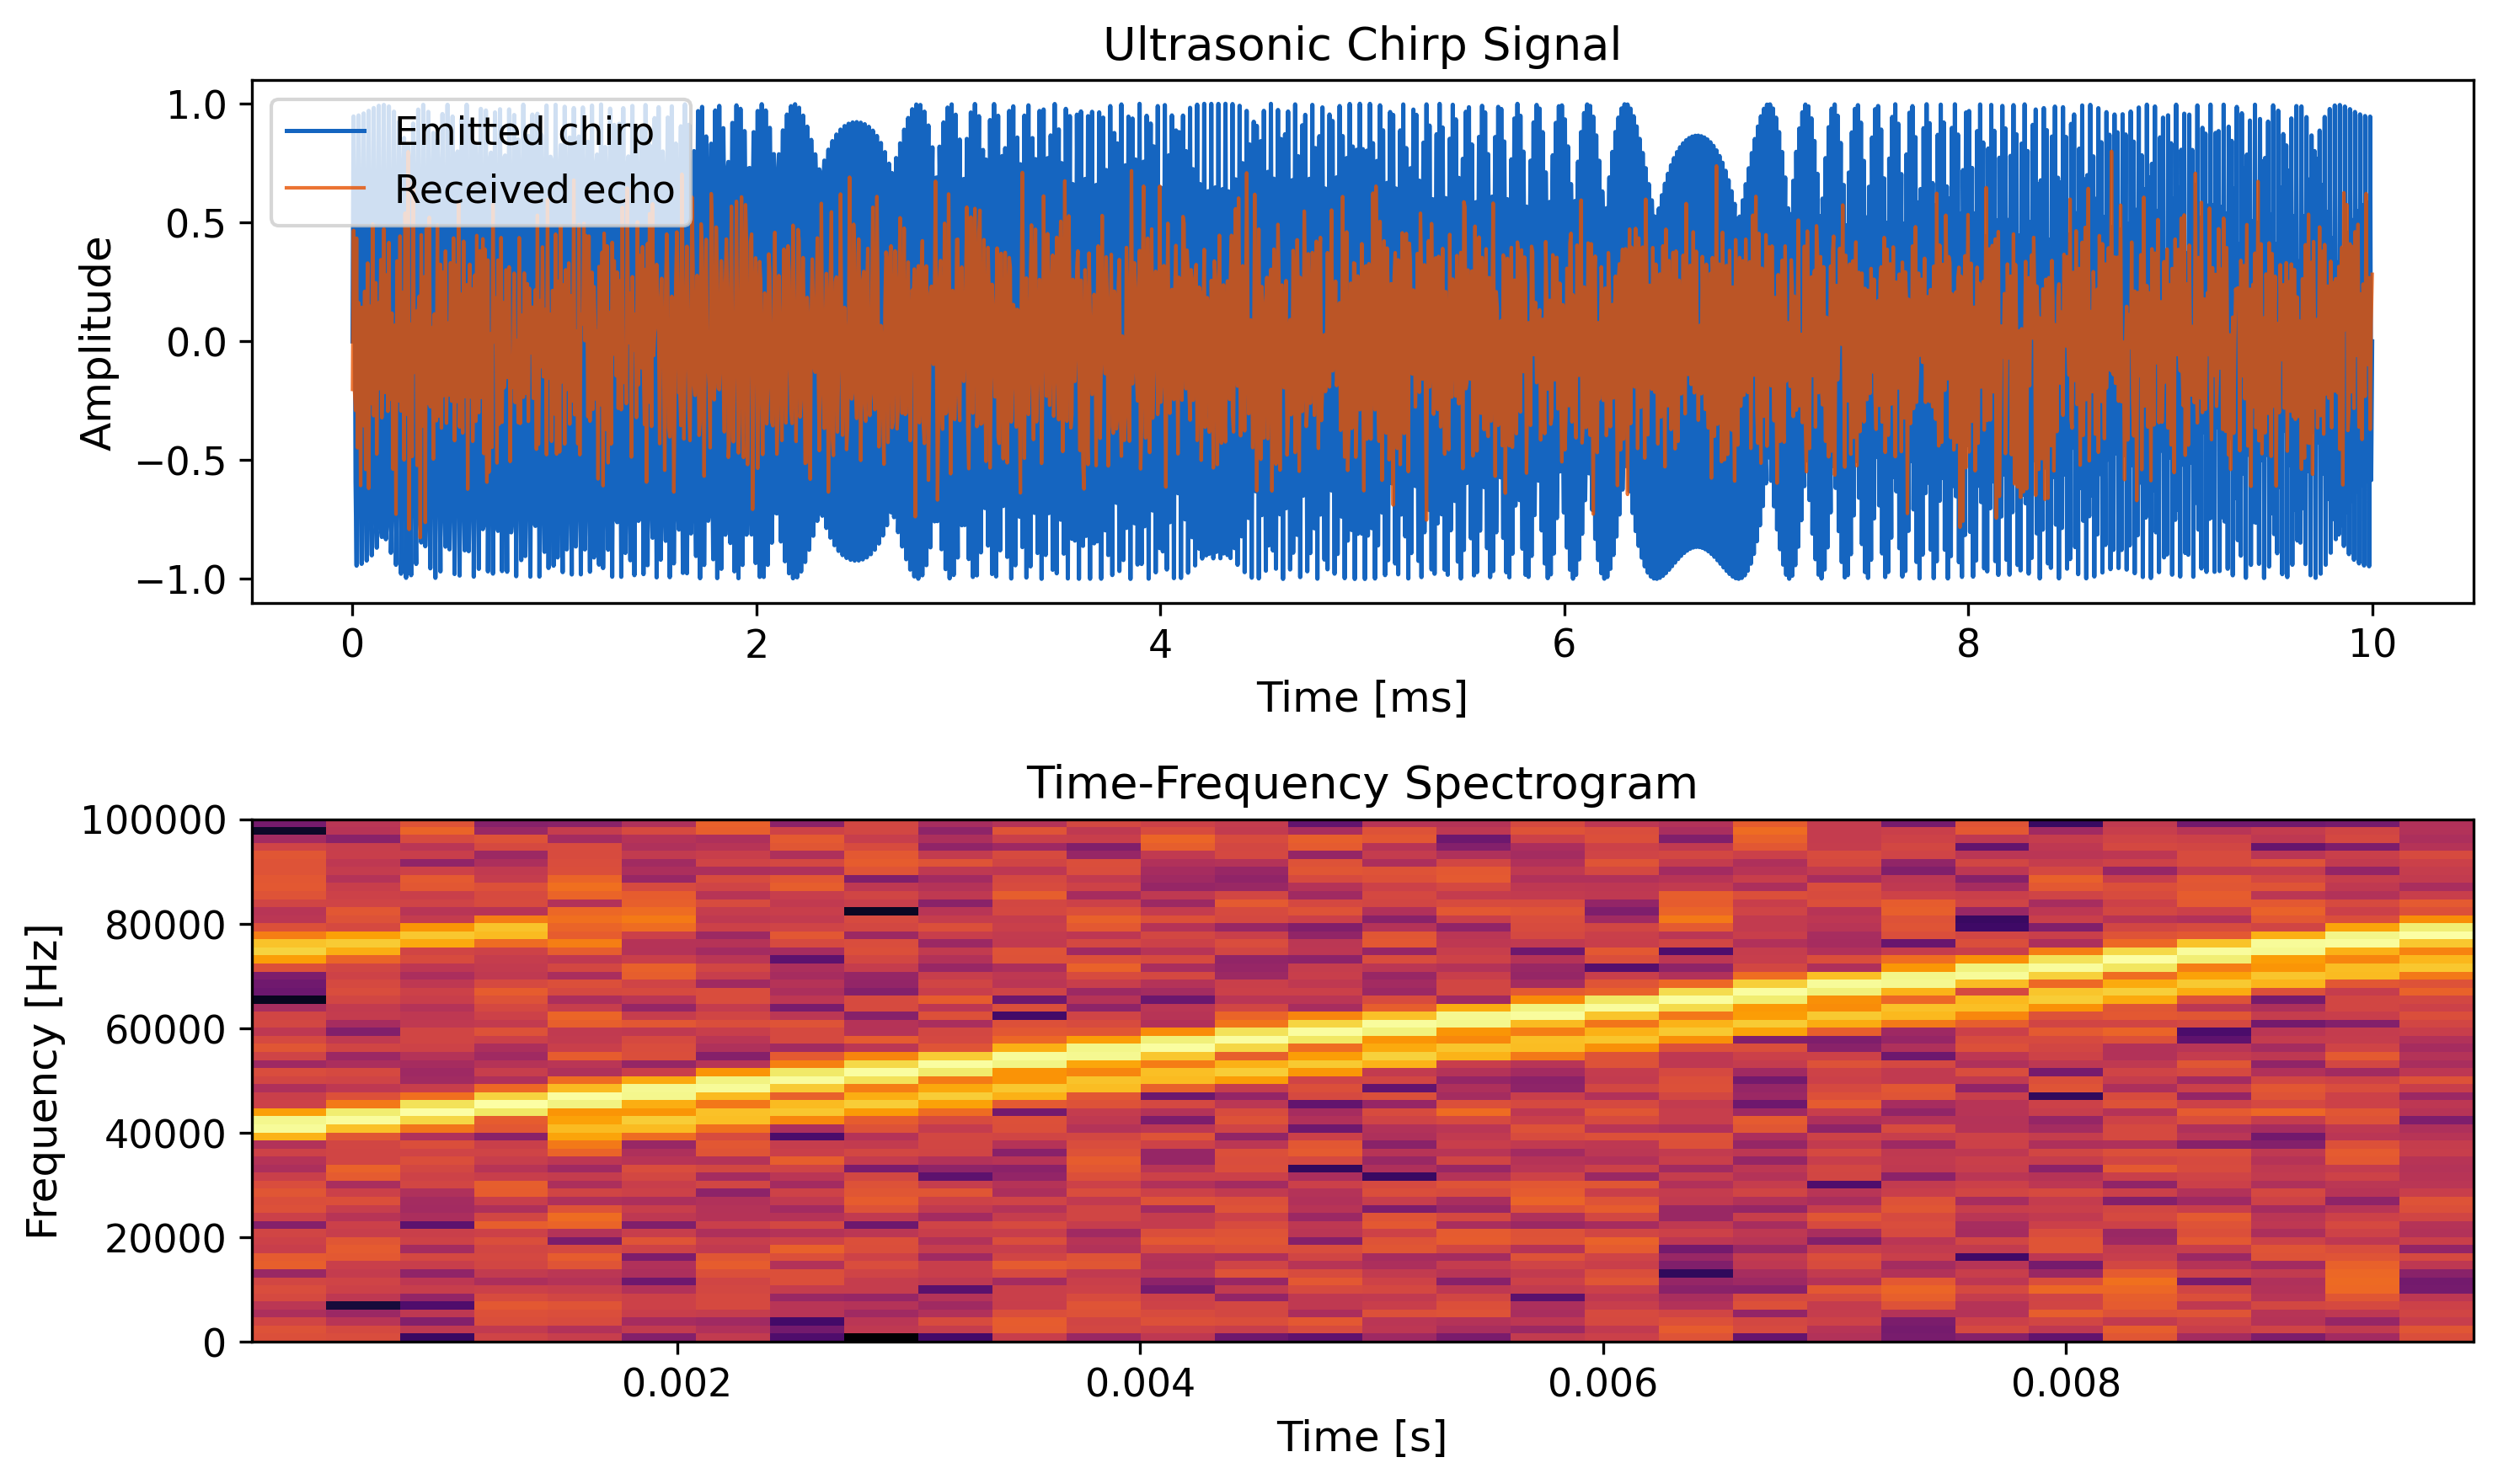
\includegraphics[width=0.95\columnwidth]{figures/fig_pit_organ_anatomy.png}
\caption{אנטומיה של איבר הגומה של הצפע הגומתי. משמאל לימין: חתך רוחבי של הראש, מבנה איבר הגומה, ומיקרוסקופיה של תאי הקולטן התרמיים. (Anatomy of the pit viper pit organ: cross-section of the head, pit organ structure, and microscopy of thermal receptor cells.)}
\label{fig:ch02_pit_organ}
\end{figure}
